\section{Design}

Whereas recent work views user threads as a fundamental language abstraction that can
be used to implement preemptible functions, we argue just the opposite.  As discussed
in Section~\ref{sec:intro}, we believe there are already a number of clear use cases
for preemptible functions in their own right, many of which are unrelated to
parallelism and therefore have no need for the scheduler, multiple kernel threads, or
synchronization to support a full threading abstraction.  To prove that our
abstraction does not compromise on expressive power, we end this section by
demonstrating how it can be trivially applied to convert an existing cooperative
userland threading library to a preemptive one.

\begin{figure}
\begin{verbatim}
struct linger {
  bool is_completion;
  union {
    void *completion;
    opaque_t continuation;
  };
};

typedef void *(*function_t)(void *);

struct linger launch(function_t func,
  uint64_t time);
  void *args);
void resume(struct linger *timed_func,
  uint64_t time);
\end{verbatim}
\caption{Core libinger (C language) interface}
\label{fig:interface}
\end{figure}

We propose an interface consisting of two functions, \texttt{launch()} and
\texttt{resume()} (Figure~\ref{fig:interface}).  Both are ordinary, structured calls
whose invocation adheres to C's standard stack discipline; there is no
continuation-style or unstructured control flow.  Client code creates a preemptible
function by passing an ordinary function (or closure) to the \texttt{launch()}
function along with an execution time cap (in microseconds).  If the function
completes on time, \texttt{launch()} propagates its result to the caller; otherwise,
it returns an opaque continuation object that the caller may later pass to
\texttt{resume()} to continue executing the function from wherever it was preempted.
Figure~\ref{fig:usage} shows a basic usage example where the caller is obligated to
perform some work after a certain amount of time (say, call a watchdog), but first
calls into some helper code with weak time bounds.  Thanks to preemptible functions,
the caller doesn't have to trust the helper to know that the watchdog will be called
in time.

\begin{figure}
\begin{verbatim}
res = launch(helper, TIMEOUT, NULL);
call_watchdog(); // Won't be delayed.
if(res.is_completion)
  // We're already done.
  return res.completion;
else
  // Give helper() some more time.
  resume(&res, TIMEOUT);
// ...
\end{verbatim}
\caption{Basic libinger usage example}
\label{fig:usage}
\end{figure}

Although the interface we propose bears some similarities to that of Scheme
engines~\cite{haynes:iucs1984}, some of our design decisions deliberately differ from
theirs:  (1) We return a structured type instead of a function, since the latter
approach would be unportable between languages.  Note that in languages with operator
overloading, it's possible to achieve the other syntax by defining the
\texttt{linger} type's function-call operator to call the \texttt{resume()} function.
(2) Because the preemptible function itself may state, we make the \texttt{linger}
type stateful as well, allowing \texttt{resume()} to mutate it in place.
(3) Instead of passing the preemptible function's return value to a separate callback
function, we return it directly from \texttt{launch()}.  This decision was made
because many modern languages have first-class tagged union (sum) types that allow
the compiler to enforce that the caller explicitly checks whether the function
completed and only accesses the appropriate side of the union.

Those familiar with futures may notice their applicability to preemptible functions
and simularity to our interface.  While each language's futures differ slightly,
preemptible function bindings can be constructed in the following trivial manner:
To create a new preemptible future, the bindings should call \texttt{launch()} with a
budget of 0 $\mu$s.  Each attempt to poll the future for a value should resolve to a
call to \texttt{resume()} with the timeout passed to poll (if allowed by the
language's API), or else previously associated with the future by other means.

The rest of this section describes the implementation of the software stack that
supports preemptible functions and fine-grained userland preemptive threading.  We
start by discussing \textit{libgotcha} (Section~\ref{sec:libgotcha}), a library that
seeks to automatically address many problems related to shared state in third-party
code.  Next, we give an aside illustrating the straightforward application of
libgotcha to provide POSIX async-signal-safety in places where it wouldn't otherwise
exist (Section~\ref{sec:statefulness}).  We then cover the \textit{libinger} library
for running preemptible functions (Section~\ref{sec:libinger}) and its interaction
with libgotcha.  Finally, we present our experience with porting a userland threading
library to libinger in order to make it preemptive (Section~\ref{sec:threading}).
Figure~\ref{fig:architecture} shows these components in the overall architecture.

\begin{figure}
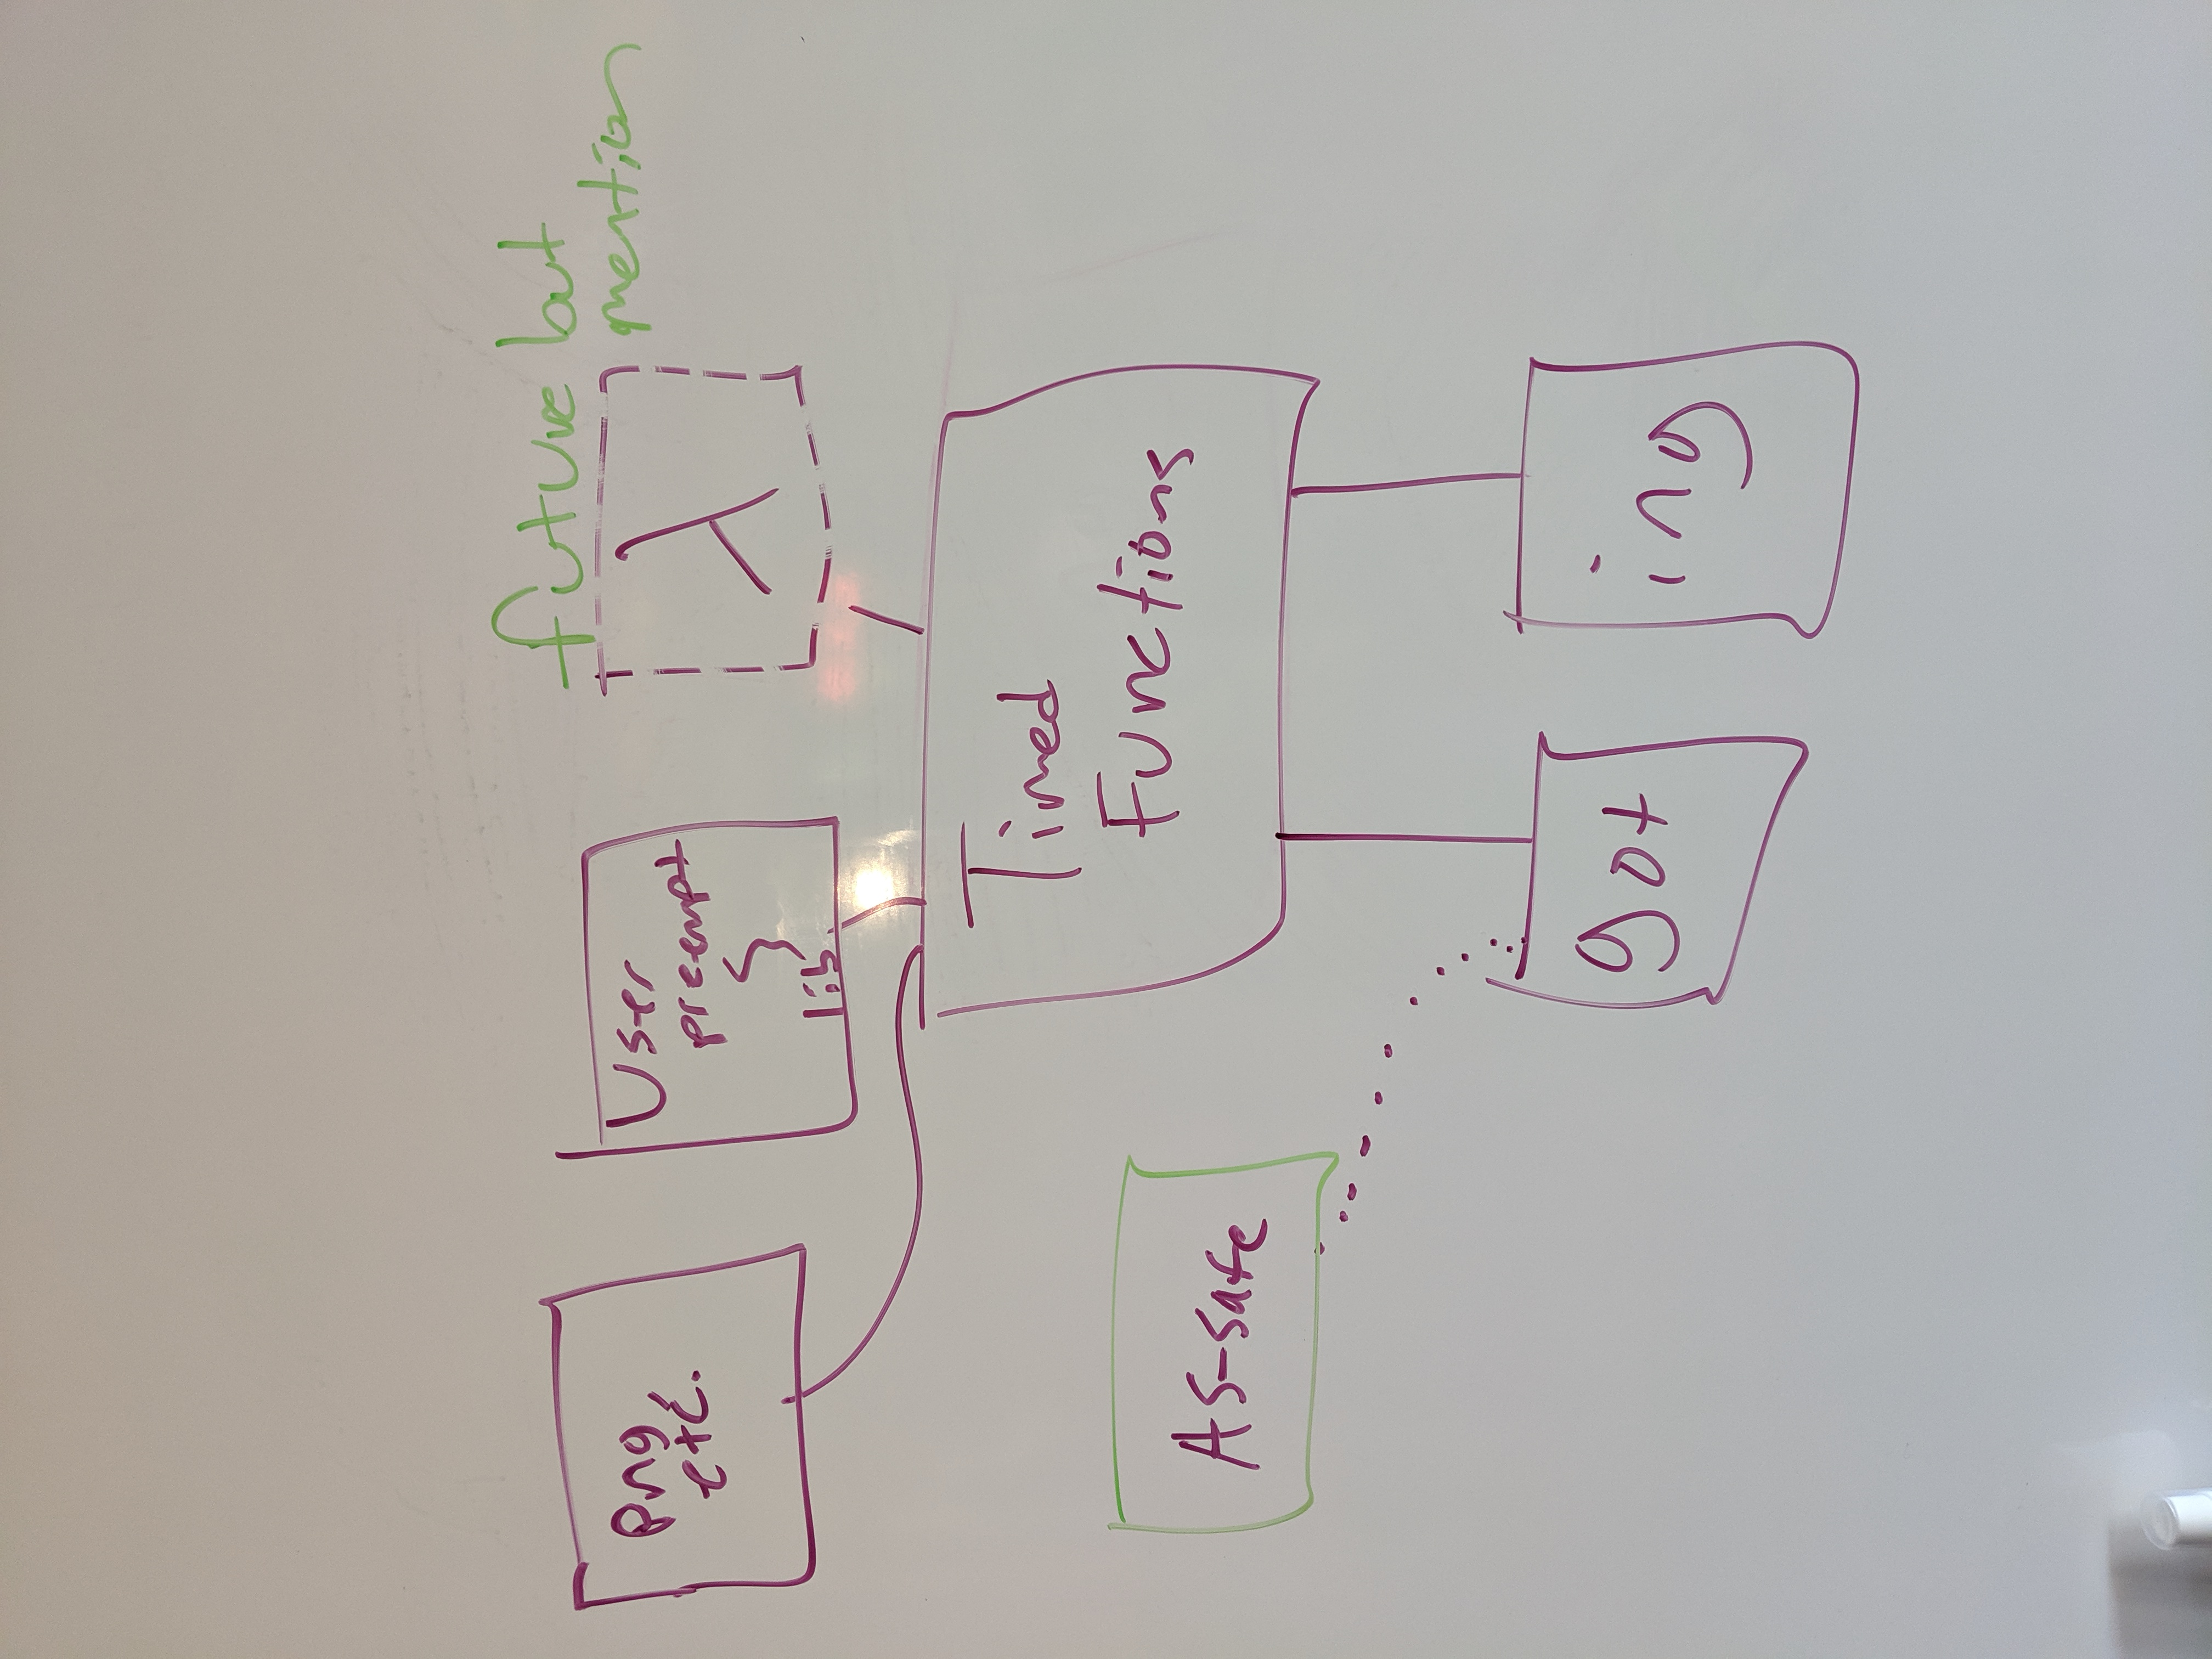
\includegraphics[width=\columnwidth,angle=270]{figs/architecture}
\caption{Architecture of preemptible functions stack}
\label{fig:architecture}
\end{figure}

\subsection{Shared state: \textit{libgotcha}}
\label{sec:libgotcha}

\subsection{Case study: Establishing AS-safety}
\label{sec:statefulness}

\subsection{Preemptible functions: \textit{libinger}}
\label{sec:libinger}

\subsection{Case study: Userland threading}
\label{sec:threading}

\solb{Discuss Table 1 from Shinjuku and its implications for our design}

\solb{Go ``also'' heap-allocates goroutine locals: \url{https://github.com/golang/go/issues/33216}}
